\documentclass[12pt, letterpaper]{article}
\usepackage{graphicx}
\graphicspath{{images/}}
\title{NMOS}
\author{}
\date{}
\begin{document}

\maketitle

\section*{Schematic}
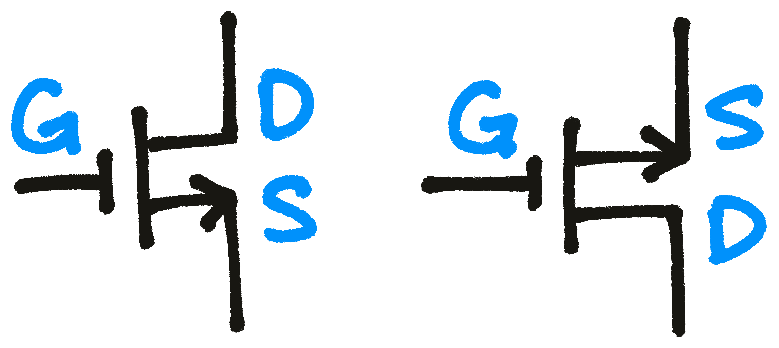
\includegraphics{symbols}

\section*{Equations}
\begin{tabular}{ l l l }
Equation & Conditions & Notes \\ 
$i_D = 0$ & $v_{GS} < V_{tn}$ & (Cutoff region) \\  
$i_D = k_n^{\prime} \left( \frac{W}{L} \right) \left( v_{OV} - \frac{1}{2} v_{DS} \right) v_{DS}$ & $v_{DS} < v_{OV}$ & (Triode region) \\
$i_D = \frac{1}{2} k_n^{\prime} \left( \frac{W}{L} \right) v_{OV}^2$ & $v_{DS} \geq v_{OV}$ & (Saturation region)
\end{tabular}

\section*{Notes}

\end{document}
